\refstepcounter{Exercise}
\clearpage\subsection*{\theExercise \ruby{郵便}{ゆうびん}番号から住所を調べるウェブページのスクレイピング}
\addtocounter{Exercise}{-1}\refstepcounter{Exercise}\label{E:postNum}
\noindent 考え方

まずは、ウェブブラウザで郵便番号から住所を調べるウェブページを見てみよう。
授業で使用したホームページを開いてください。
\textbf{({\textasciitilde}/08/links.html)}

郵便番号から住所を調べるをクリックします。
\begin{center}
  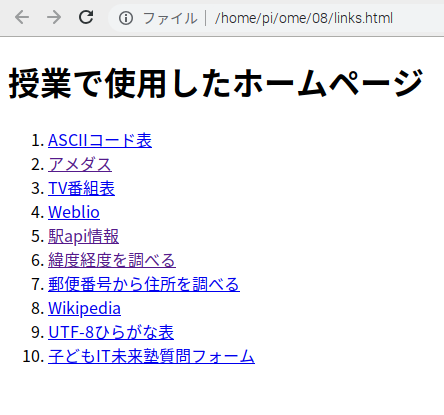
\includegraphics[width=7.181cm]{textbook-img017.png}
\end{center}

郵便番号から住所を調べるウェブページが開きます。
郵便番号に対応する住所ががHTMLのようなページで表示されます。

今回取得する情報は都道府県、市町村です。

\begin{center}
  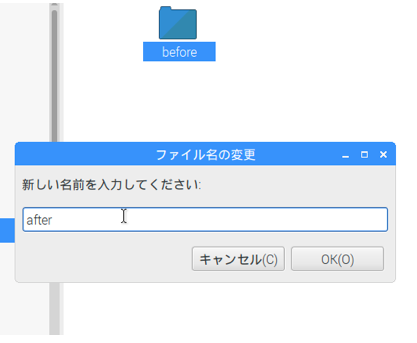
\includegraphics[width=15.492cm]{textbook-img055.png}
\end{center}

\clearpage
まずはプログラムを動かしてみましょう。

ターミナルを開いて

hsed

と実行してスクリプトエディタを開きます。



\begin{center}
  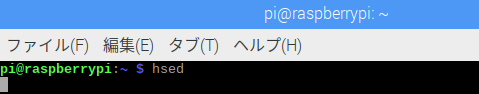
\includegraphics[width=\textwidth]{textbook-img013.png}
\end{center}
HSPスクリプトエディタが開くので

ファイル → 開く.. \ をクリックして\textbf{{\textasciitilde}/08/zipcode.hsp}を開きます。

プログラムが表示されます。

\begin{center}
  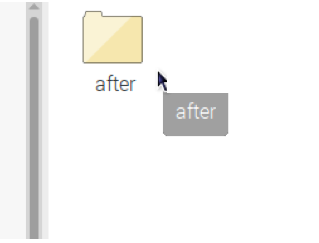
\includegraphics[width=13.951cm]{textbook-img056.png}
\end{center}


\clearpage
F5を押して実行してみましょう。実行結果はターミナルに表示されます

\begin{center}
  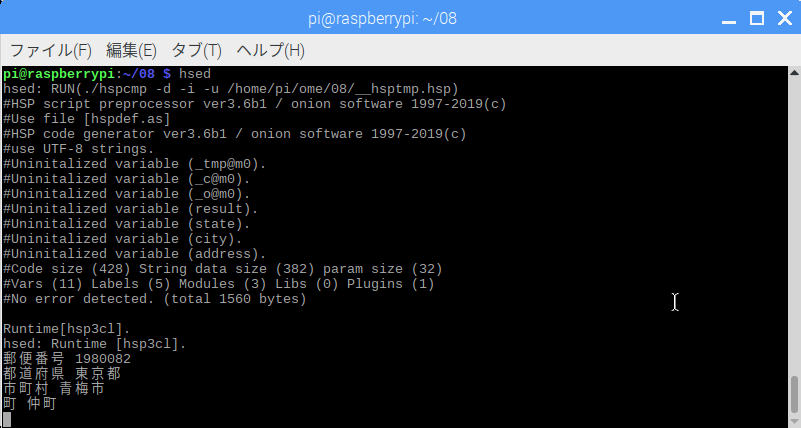
\includegraphics[width=0.8\textwidth]{textbook-img057.png}
\end{center}
ブラウザの表示とプログラムの実行結果を比べてみてください。
郵便番号に対応する都道府県、市町村が表示されているのがわかります。

\begin{center}
  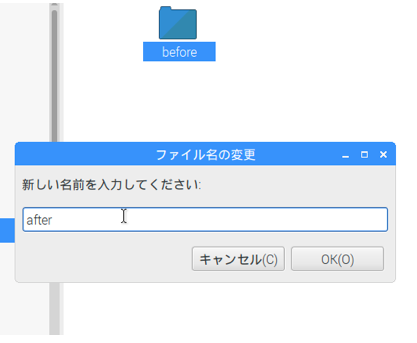
\includegraphics[width=0.8\textwidth]{textbook-img055.png}
\end{center}

\refstepcounter{Question}
\subsection*{\theQuestion\label{Q:postNum}}
codeの郵便番号を変更してみよう
\ \ 例: 198-0082
青梅\ruby{佐藤財団}{さとうざいだん}の郵便番号

\begin{center}
\begin{boxedminipage}{10.927cm}
\begin{enumerate}
\item code = “1980082”
\end{enumerate}
\end{boxedminipage}
\end{center}

\refstepcounter{Exercise}
\clearpage
\subsection*{\theExercise Wikipediaのスクレイピング}
\addtocounter{Exercise}{-1}\refstepcounter{Exercise}\label{E:wikipedia}
\noindent 考え方

まずは、ウェブブラウザでWikipediaを見てみよう。
授業で使用したホームページを開いてください。
\textbf{({\textasciitilde}/08/links.html)}

Wikipediaをクリックします。
\begin{center}
  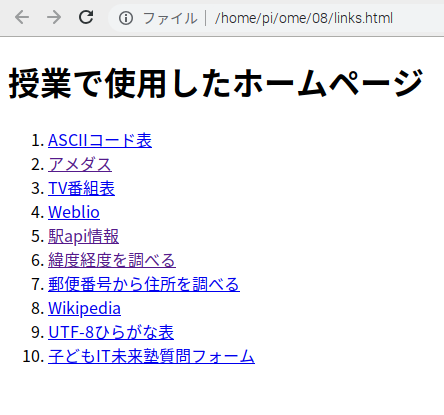
\includegraphics[width=0.5\textwidth]{textbook-img017.png}
\end{center}

Wikipediaが開きます。
このページの検索欄に検索したいワードを入れて検索をすると結果がでてきます。
まずは、適当に検索してみましょう。
\begin{center}
  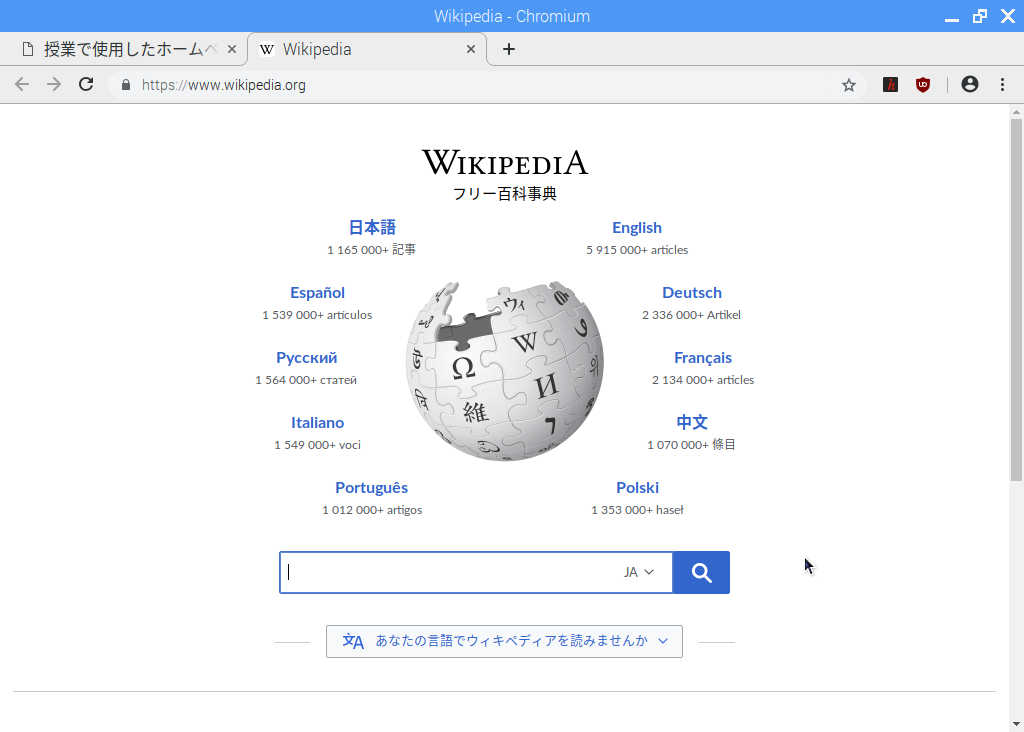
\includegraphics[width=0.8\textwidth]{textbook-img058.png}
\end{center}

\clearpage
試しに”Raspberry
Pi”と検索してみました。
結果の画面はこのような感じです。

\begin{center}
  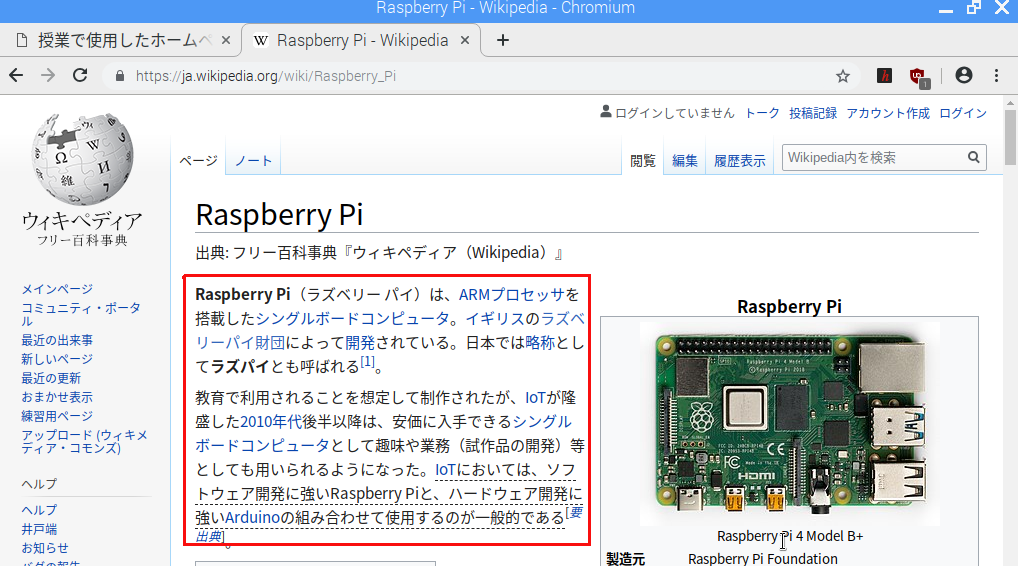
\includegraphics[width=0.9\textwidth]{textbook-img059.png}
\end{center}
今回取得する情報はラズベリーパイの\ruby{概要}{がいよう}です。

まずはプログラムを動かしてみましょう。

ターミナルを開いて

hsed

と実行してスクリプトエディタを開きます。



\begin{center}
  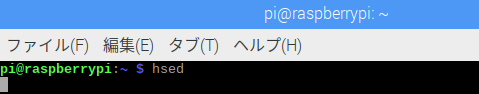
\includegraphics[width=0.9\textwidth]{textbook-img013.png}
\end{center}

\clearpage
HSPスクリプトエディタが開くので

\bigskip

ファイル → 開く..\ をクリックして\textbf{{\textasciitilde}/08/wikipedia.hsp}を開きます。

プログラムが表示されます。

\begin{center}
  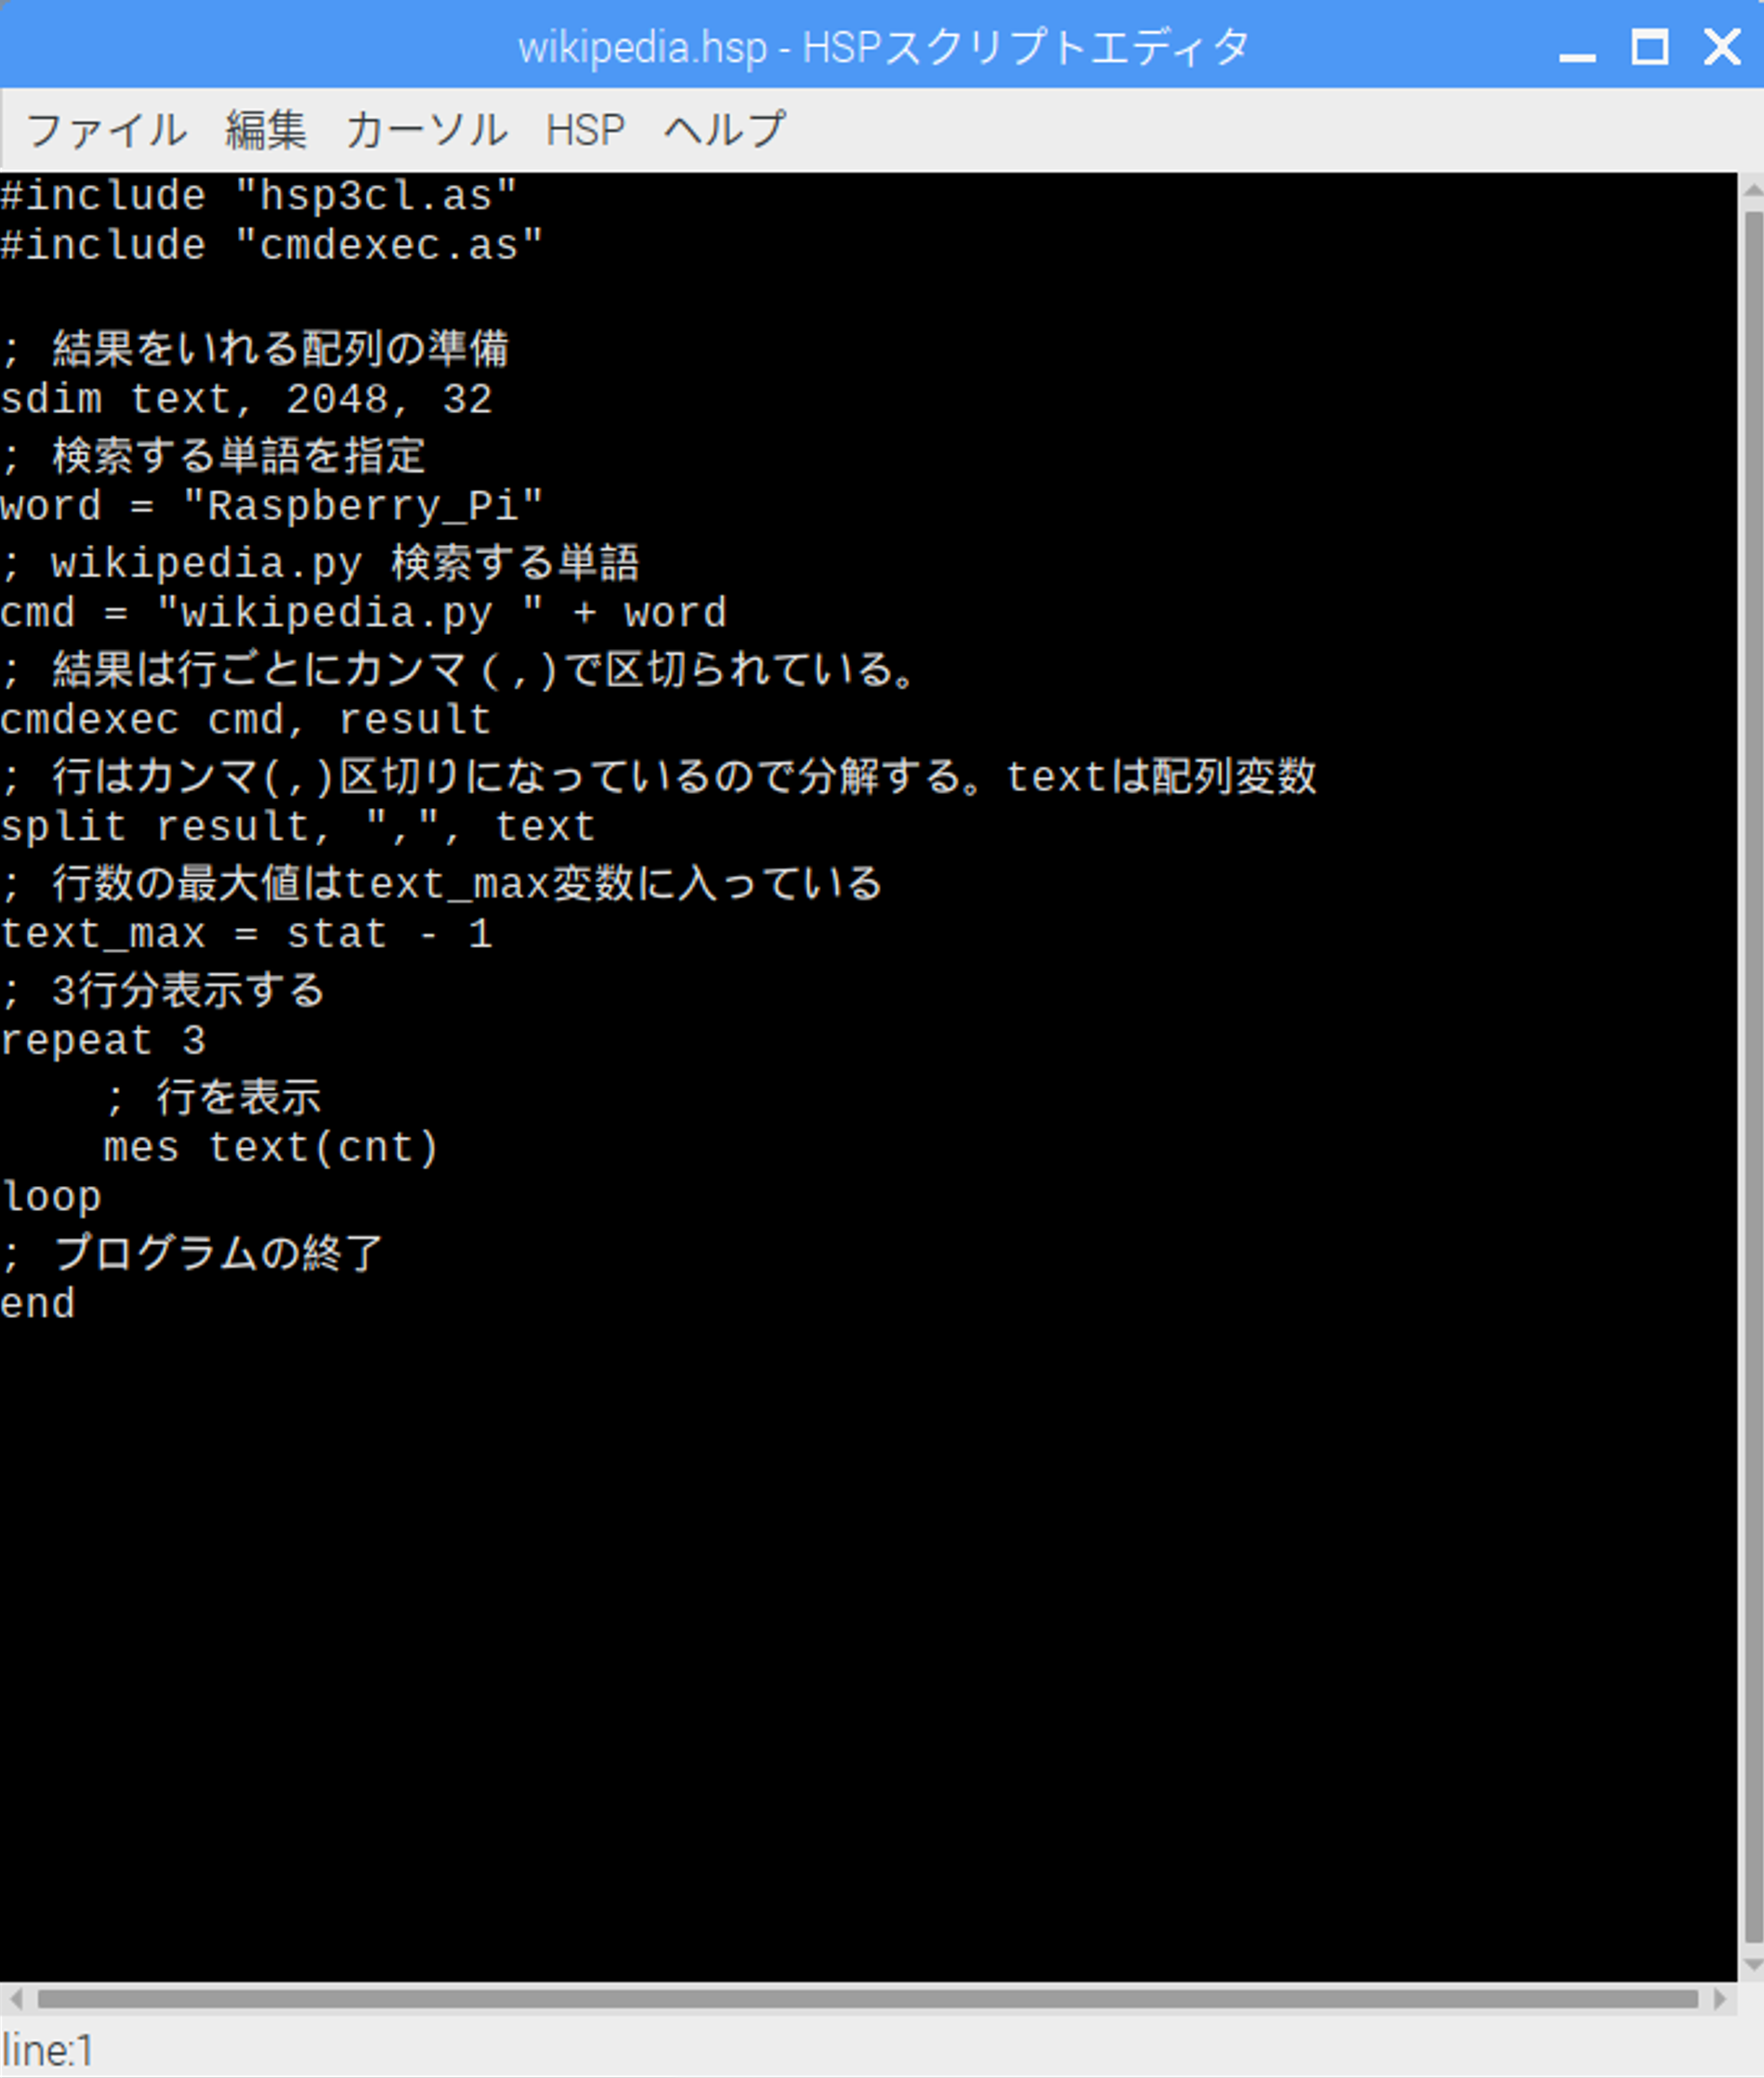
\includegraphics[width=\textwidth]{img00060.png}
\end{center}

\clearpage
F5を押して実行してみましょう。実行結果はターミナルに表示されます
\begin{center}
  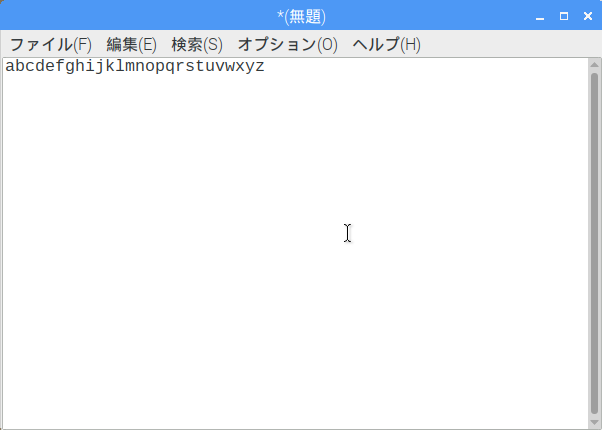
\includegraphics[width=\textwidth]{textbook-img061.png}
\end{center}
ブラウザの表示とプログラムの実行結果を比べてみてください。
検索用語(Raspberry
Pi)の概要がWikipediaからとれました。

\begin{center}
  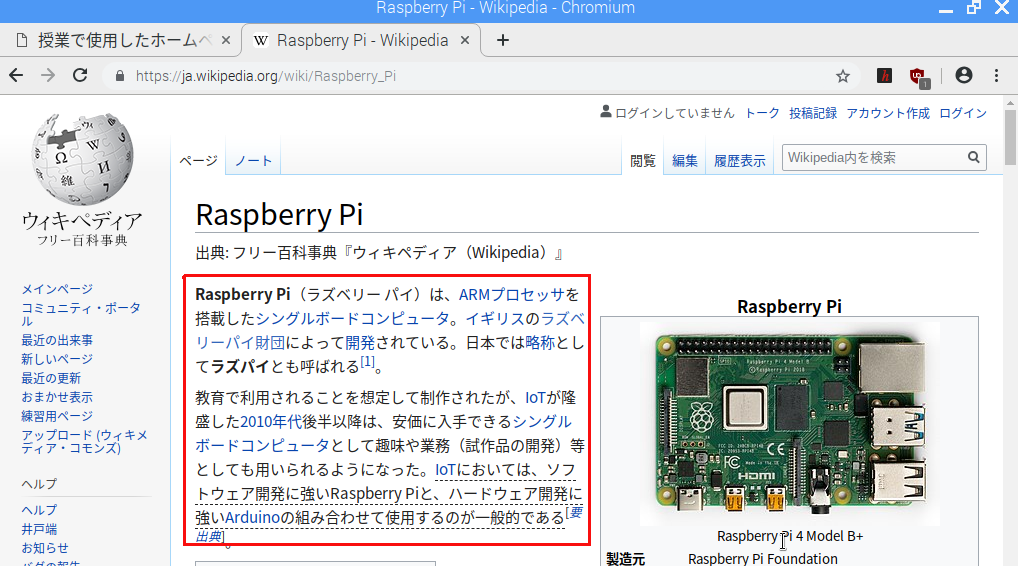
\includegraphics[width=\textwidth]{textbook-img059.png}
\end{center}

\refstepcounter{Question}
\subsection*{\theQuestion\label{Q:wikipedia}}
wordを自分の検索したい単語に変えてみよう。

\ \ HINT:まずは、Wikipediaで検索したい単語を検索をしてみて、ページを開きましょう。

URLの

http://ja.wikipedia.org/wiki/*******

wiki/より後にある文字列をwordに入れます。
\begin{center}
  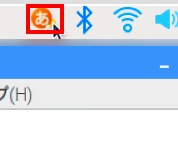
\includegraphics[width=0.9\textwidth]{textbook-img062.png}
\end{center}
例えば、

word = “フランシスコ・ザビエル”

検索用語によってはページがWikipediaにないことがあります。
